\chapter{Лекция 7. Код Прюфера (обратная задача). Остовные деревья. Алгоритм Прима}

% ============================================================
% ОБРАТНАЯ ЗАДАЧА КОДА ПРЮФЕРА (стр. 17, dir2 стр. 5)
% ============================================================

\subsection*{Обратная задача кода Прюфера}

\textbf{Дано:}
$V = \{v_1, \ldots, v_n\}$,\quad
$\operatorname{Pruf}(G) = \{v_{i_1}, \ldots, v_{i_{n-2}}\}$.

\textbf{Восстановить} $G$.

\textbf{Step:} выбор $\min$ из $(V \setminus \operatorname{Pruf}(G)) = v_k$; соединяем:
$e = v_k v_{i_s}$, удаляем $v_k$ из $V$, $v_{i_s}$ из $\operatorname{Pruf}(G)$
\quad ($v_{i_s}$ --- $s$-й элемент кода, $s$ --- номер шага).

\textbf{Замечание:} в процессе не обязательно должно быть дерево, а в конце --- обязательно.

% ============================================================
% Пример обратной задачи (стр. 18, dir2 стр. 6)
% ============================================================

\medskip
\noindent\textbf{Пример.}

$V = \{A, B, C, D, E, F, H, I, J\}$,\quad
$\operatorname{Pruf}(G) = \{D, A, A, F, H, A, J\}$.

% Граф: p18-example-1.graph
\grfig{figures/p18-example-1.pdf}{Обратная задача Прюфера}

% ============================================================
% ТЕОРЕМА КЭЛИ (стр. 18, dir2 стр. 6)
% ============================================================

\subsection*{Теорема Кэли}

$V = \{v_1, \ldots, v_n\}$; сколько $\exists$ различных помеченных деревьев?

$|\operatorname{Pruf}(G)| = n - 2 \;\Rightarrow\; n^{n-2}$ помеченных деревьев.

\begin{statement}{Теорема Кэли (о количестве помеченных деревьев)}{cayley}
Количество различных помеченных деревьев на $n$ вершинах равно $n^{n-2}$.
\end{statement}

\begin{proof}
Построим биекцию между помеченными деревьями на $n$ вершинах и
последовательностями длины $n - 2$ из элементов $V$ --- это в точности
код Прюфера.

\textbf{Код корректно определён.} Прямой алгоритм (лекция 6) на каждом
шаге удаляет минимальный лист (у дерева с $\ge 2$ вершинами лист всегда
есть) и делает ровно $n - 2$ записи --- любому дереву отвечает ровно одна
последовательность $\operatorname{Pruf}(G) \in V^{n-2}$.

\textbf{Инъективность и сюръективность.} Обратный алгоритм (выше) по
\emph{любой} последовательности $p \in V^{n-2}$ строит граф: на каждом
шаге к минимальной вершине, не встречающейся в остатке кода и ещё не
использованной, проводится ребро к первому элементу кода. Получается
ровно $n - 1$ ребро, и построенный граф связен и ацикличен (каждый шаг
присоединяет <<новый лист>> к остальной части), т.\,е. дерево. Прямой
проверкой видно, что обратный алгоритм восстанавливает исходное дерево
по его коду, а прямой алгоритм, применённый к дереву, построенному по
последовательности $p$, возвращает $p$. Значит, соответствие ---
биекция.

Последовательностей длины $n - 2$ из $n$ символов ровно $n^{n-2}$,
следовательно, столько же и помеченных деревьев.
\end{proof}

% ============================================================
% РЁБЕРНО-ВЗВЕШЕННЫЕ ГРАФЫ. MIN ОСТОВНОЕ ДЕРЕВО (стр. 18, dir2 стр. 6)
% ============================================================

\subsection*{Рёберно-взвешенные графы. Минимальное остовное дерево}

\begin{defn}{Рёберно-взвешенный граф}{weighted-graph}
$G(V, E)$ --- (рёберно-)взвешенный:

$\exists\, \sigma\colon E \to W$,

где $W$ --- некоторое упорядоченное мн-во
с операциями, зависящими от задачи.

\textbf{NB:} $W$ --- нижняя упорядоченная мн-во.
\end{defn}

$G(V, E)$ --- неориент., н.\,у.\,о. --- связный.

$\sigma\colon E \to \mathbb{R}$.

\begin{defn}{Остов (каркас)}{spanning-tree-def}
\textbf{Остов} (скелет, каркас) --- связный подграф в $G$, являющийся деревом и содержащий все вершины $G$.
\end{defn}

\begin{defn}{Остовное дерево}{spanning-tree}
$G(V, E)$ --- \textbf{остовное дерево} $G$: $T$ --- дерево и остов.

Если граф --- не дерево, то остовов несколько.
\end{defn}

% Пример: треугольник — 3 остова

\begin{defn}{Минимальное остовное дерево}{mst}
$G(V, E)$ --- связный, взвешенный.

$\sigma\colon E \to \mathbb{R}$.

Минимальное остовное дерево $G$:
$T_G\colon \displaystyle\sum_{\substack{(v,\hat{v}) \in T \\ e \in \hat{E}}} \sigma(e) \longrightarrow \min$
по всем $T$ для $G$.
\end{defn}

% ============================================================
% Жадные алгоритмы (стр. 19, dir2 стр. 7)
% ============================================================

\medskip
\textbf{Жадные алгоритмы} --- алгоритмы, оптимальные только в рамках одного шага.

% Пример контрпримера жадности:
% Граф: p19-example-1.graph
\grfig{figures/p19-example-1.pdf}{Жадный алг.: контрпример 1}

% Ещё пример:
% Граф: p19-example-2.graph
\grfig{figures/p19-example-2.pdf}{Жадный алг.: контрпример 2}

% ============================================================
% АЛГОРИТМ ПРИМА (стр. 19, dir2 стр. 7)
% ============================================================

\subsection*{Алгоритм построения min остовного дерева}

$G(V, E)$, $\sigma\colon E \to \mathbb{R}$, н.\,у.\,о. --- связный.

\begin{algo}{Алгоритм Прима}{prim}

\textbf{Инициализация:} $\operatorname{start} \in V$ (любая вершина);
дерево $T = \{\operatorname{start}\}$.

\textbf{Step:} среди всех рёбер, соединяющих уже выбранную вершину с ещё
не выбранной, берём ребро $e$ с минимальным весом $\sigma(e)$; добавляем
его (и новую вершину) в $T$. Новая вершина присоединяется не обязательно
к последней --- к \emph{любой} из уже выбранных. Повторяем, пока $T$ не
охватит все вершины ($n - 1$ ребро).

\medskip
\noindent\textbf{Пример} (старт из $J$):

% Граф: p19-prim-example-1.graph
\grfig[0.55]{figures/p19-prim-example-1.pdf}{Алг. Прима: взвешенный граф 9 вершин}

\medskip
\begin{center}
\begin{tabular}{c|c|c|l}
$V$ & $e$ & $\sum \sigma(e)$ & комментарий \\ \hline
$J$  & ---     & 0  & старт \\
$I$  & $IJ(3)$ & 3  & единственное ребро из $J$ \\
$D$  & $DI(1)$ & 4  & $DI(1) < IF(2)$ \\
$F$  & $IF(2)$ & 6  & $IF(2) < AD(4) < DH(5) = DF(5) < \ldots$ \\
$A$  & $AD(4)$ & 10 & $AD(4) < DH(5) < FH(6) < \ldots$ \\
$H$  & $DH(5)$ & 15 & $DH(5) < AB(6) = FH(6) < DC(7)$ \\
$B$  & $AB(6)$ & 21 & $AB(6) < DC(7) < BD(9)$ \\
$C$  & $BC(1)$ & 22 & после прихода $B$ открылось ребро $BC(1)$ \\
$E$  & $CE(8)$ & 30 & единственное ребро к последней вершине $E$ \\
\end{tabular}
\end{center}

\medskip
Минимальное остовное дерево: $IJ, DI, IF, AD, DH, AB, BC, CE$;
суммарный вес $\sum \sigma = 30$.

\medskip
\noindent\textbf{Работа алгоритма по шагам} (выбранные рёбра --- зелёные,
текущее добавляемое --- оранжевое, недоступные пока рёбра --- серые):

\begin{center}\begin{tabular}{ccc}
\shortstack{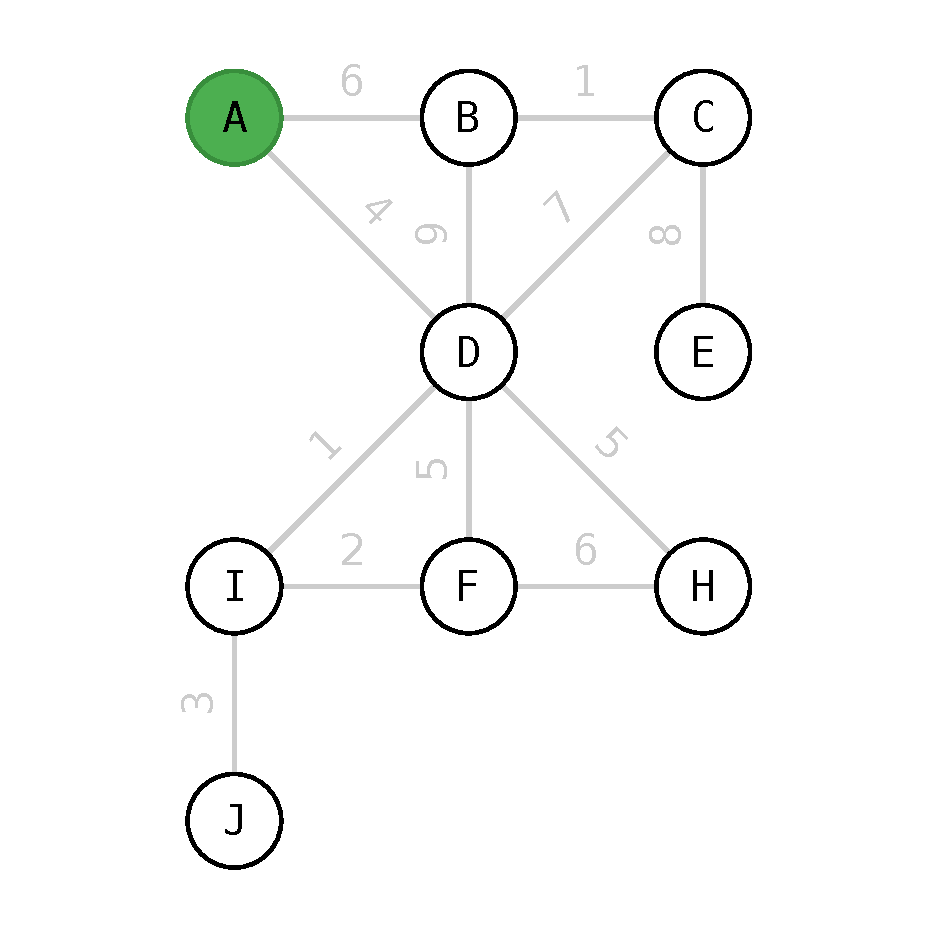
\includegraphics[width=0.30\textwidth]{python/lec07/prim/prim-0.pdf}\\[2pt]{\scriptsize Шаг 0. Старт: $T=\{J\}$}} &
\shortstack{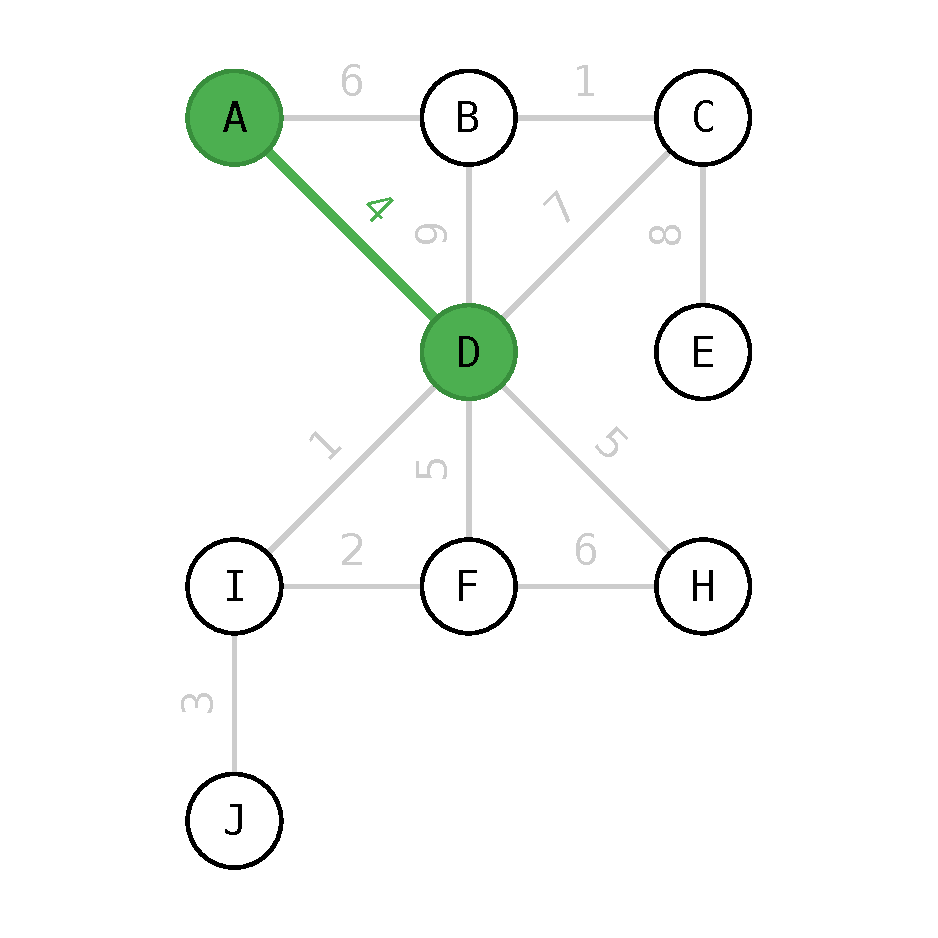
\includegraphics[width=0.30\textwidth]{python/lec07/prim/prim-1.pdf}\\[2pt]{\scriptsize Шаг 1. $+IJ(3)$, $\Sigma=3$}} &
\shortstack{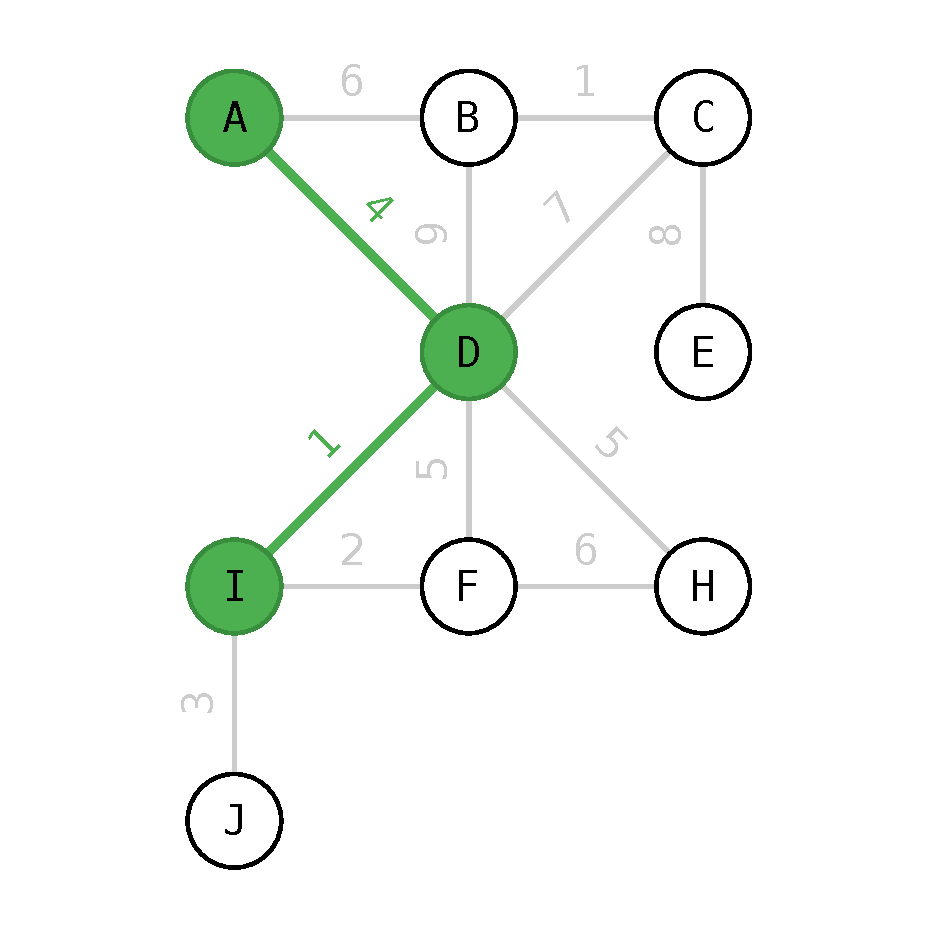
\includegraphics[width=0.30\textwidth]{python/lec07/prim/prim-2.pdf}\\[2pt]{\scriptsize Шаг 2. $+DI(1)$, $\Sigma=4$}} \\
\end{tabular}\end{center}
\begin{center}\begin{tabular}{ccc}
\shortstack{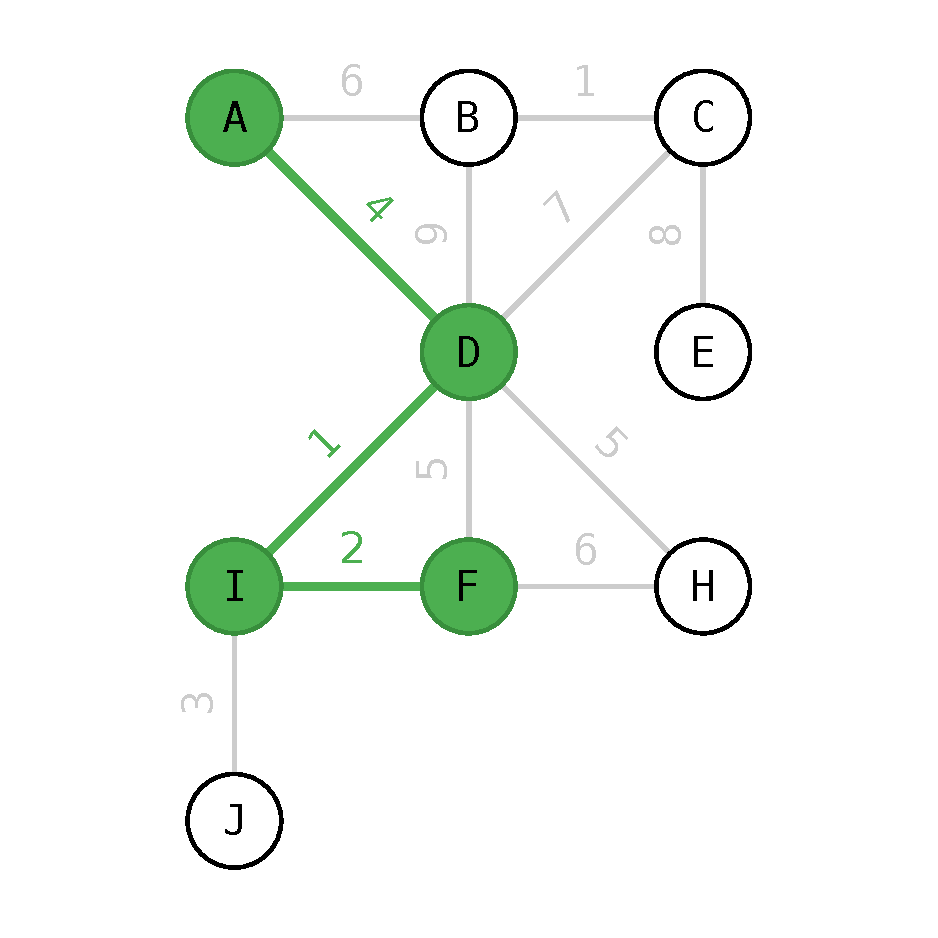
\includegraphics[width=0.30\textwidth]{python/lec07/prim/prim-3.pdf}\\[2pt]{\scriptsize Шаг 3. $+IF(2)$, $\Sigma=6$}} &
\shortstack{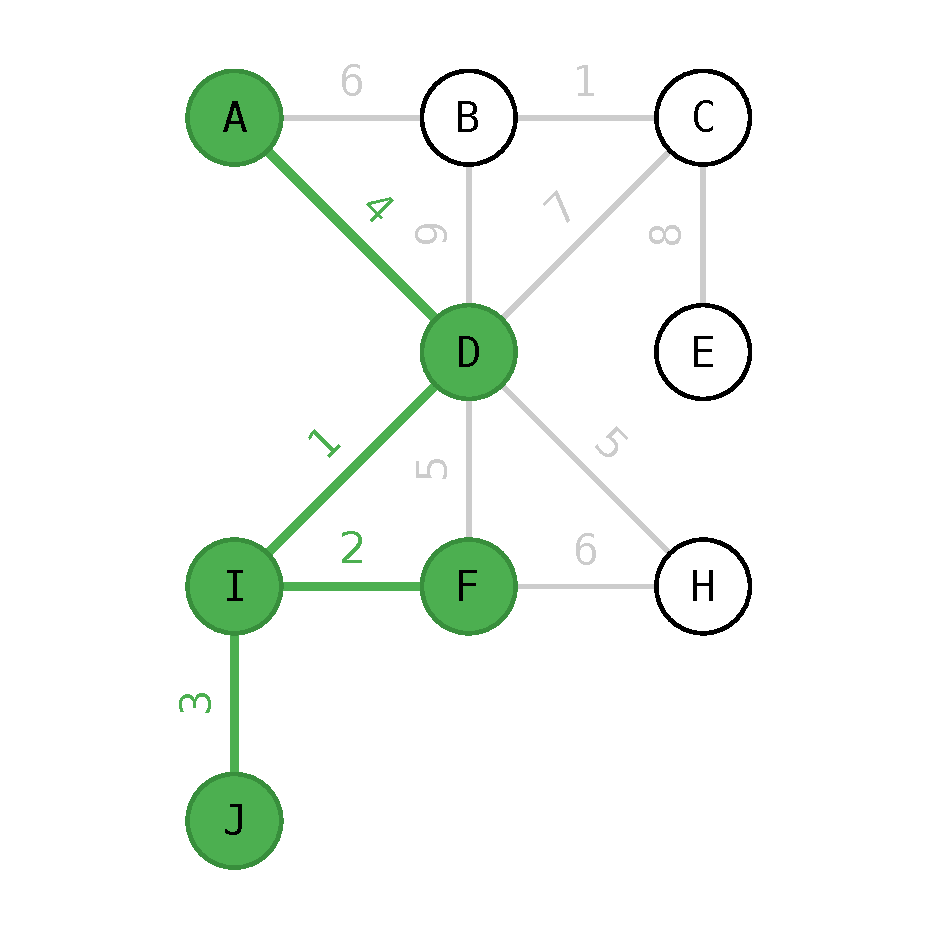
\includegraphics[width=0.30\textwidth]{python/lec07/prim/prim-4.pdf}\\[2pt]{\scriptsize Шаг 4. $+AD(4)$, $\Sigma=10$}} &
\shortstack{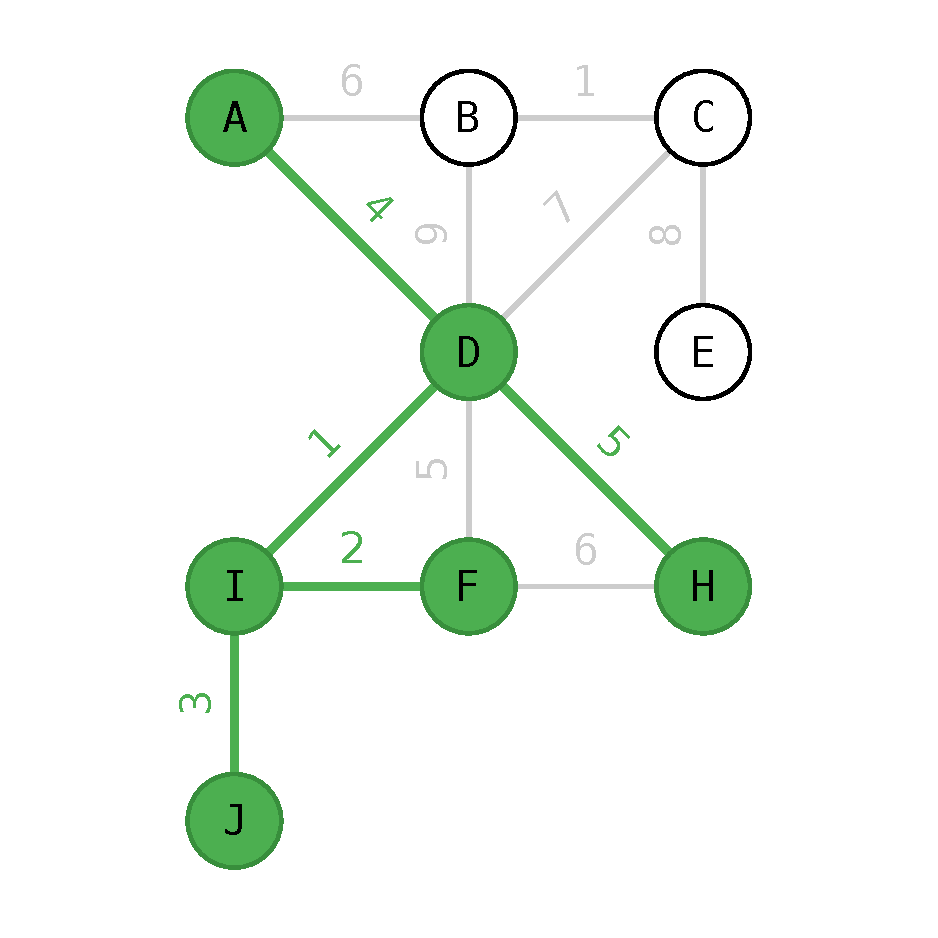
\includegraphics[width=0.30\textwidth]{python/lec07/prim/prim-5.pdf}\\[2pt]{\scriptsize Шаг 5. $+DH(5)$, $\Sigma=15$}} \\
\end{tabular}\end{center}
\begin{center}\begin{tabular}{ccc}
\shortstack{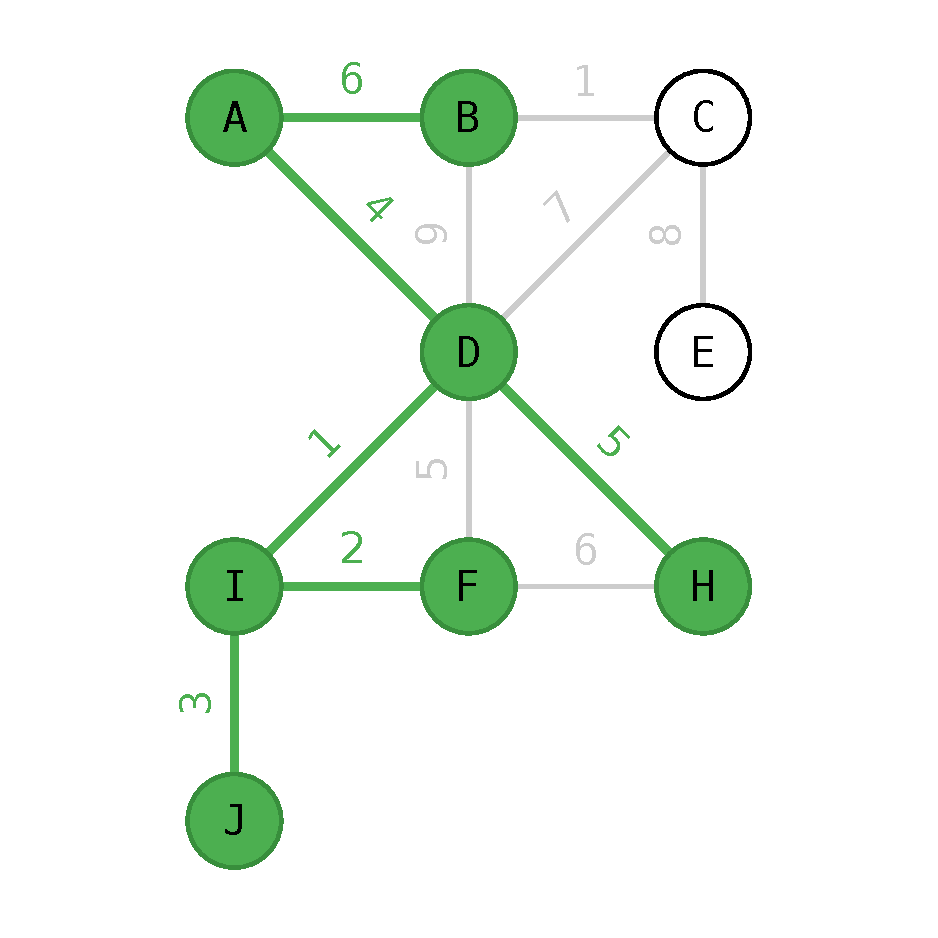
\includegraphics[width=0.30\textwidth]{python/lec07/prim/prim-6.pdf}\\[2pt]{\scriptsize Шаг 6. $+AB(6)$, $\Sigma=21$}} &
\shortstack{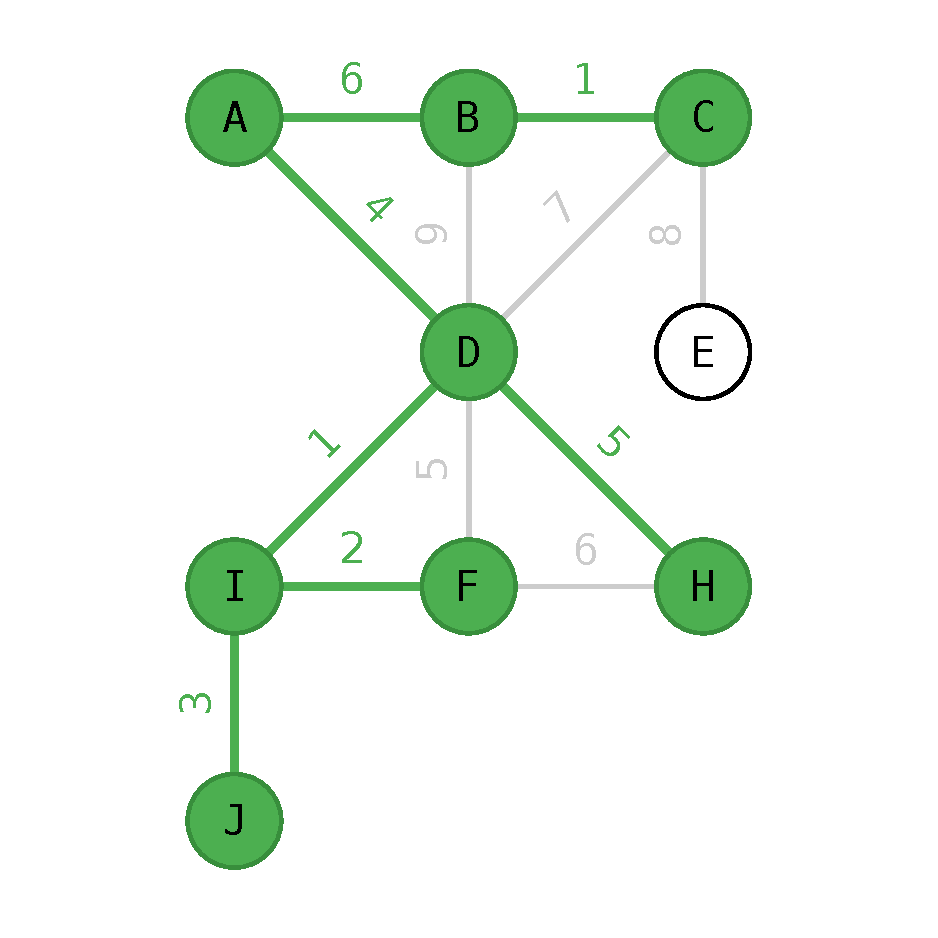
\includegraphics[width=0.30\textwidth]{python/lec07/prim/prim-7.pdf}\\[2pt]{\scriptsize Шаг 7. $+BC(1)$, $\Sigma=22$}} &
\shortstack{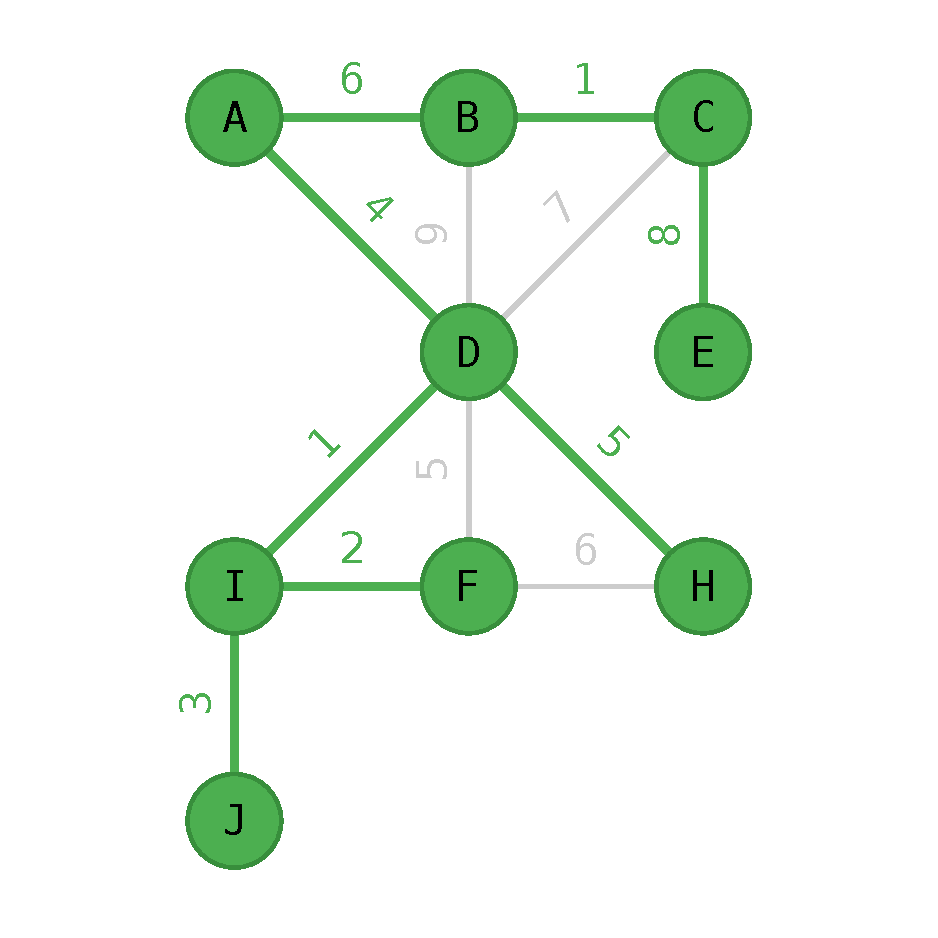
\includegraphics[width=0.30\textwidth]{python/lec07/prim/prim-8.pdf}\\[2pt]{\scriptsize Шаг 8. $+CE(8)$, $\Sigma=30$}} \\
\end{tabular}\end{center}
\begin{center}
\shortstack{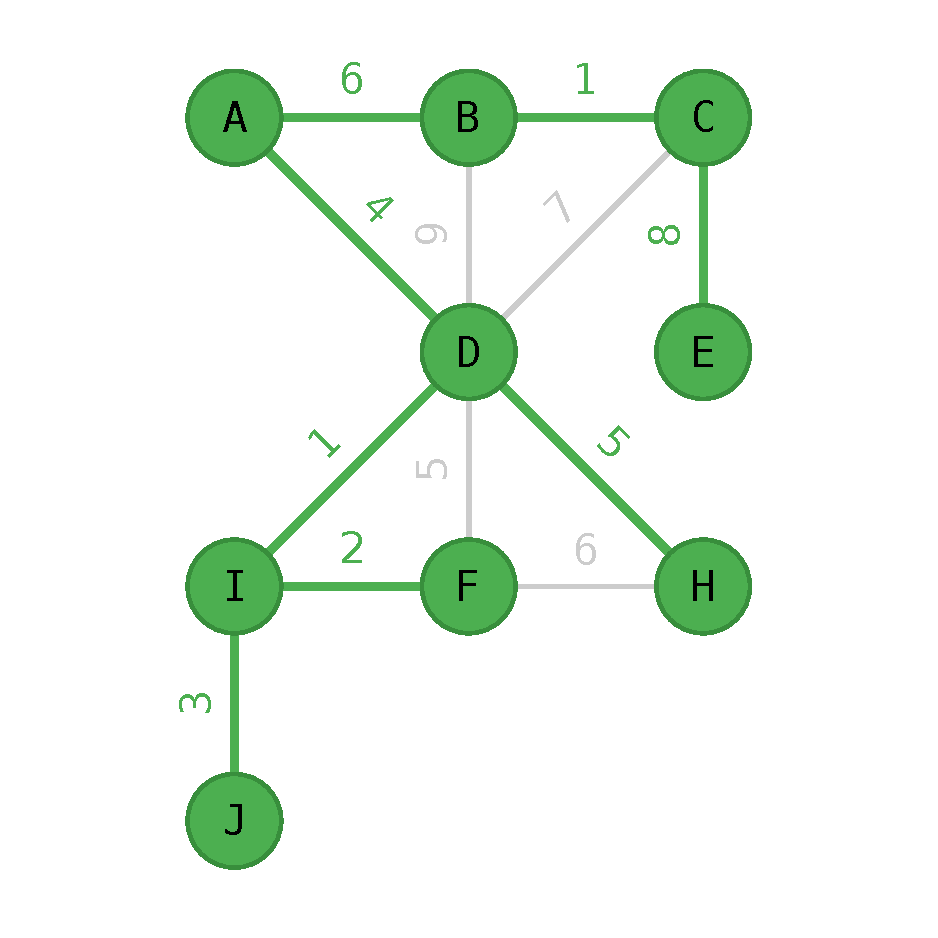
\includegraphics[width=0.32\textwidth]{python/lec07/prim/prim-9.pdf}\\[2pt]{\scriptsize Шаг 9. Остов построен, $\Sigma = 30$}}
\end{center}

\medskip
\textbf{Замечание.} Если все веса рёбер различны, минимальное остовное
дерево единственно --- и алгоритм Прима находит именно его независимо
от выбора стартовой вершины.
\end{algo}

% ============================================================
\begin{task}{Минимальное остовное дерево: алгоритм Прима}{prim-task}
\textbf{Условие.} Дан неориентированный взвешенный граф на вершинах
$A,B,C,D,E,F$ с рёбрами
\[
  AB=4,\quad AC=2,\quad BC=5,\quad BD=10,\quad CE=3,\quad ED=6,\quad EF=7,\quad DF=11.
\]
Постройте минимальное остовное дерево алгоритмом Прима, начиная с вершины $A$.
Укажите порядок включения рёбер и суммарный вес.

\begin{center}
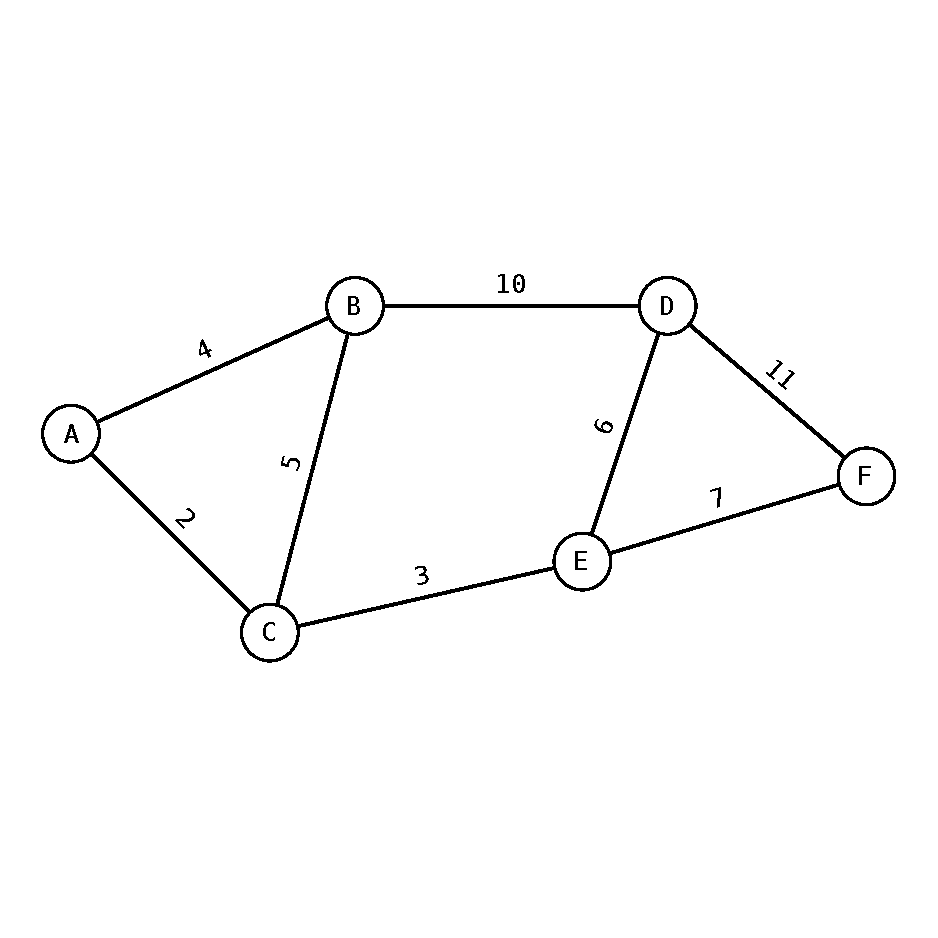
\includegraphics[width=0.5\textwidth]{figures/task-prim-1.pdf}
\end{center}

\textbf{Решение.} Алгоритм Прима выращивает дерево из одной вершины, добавляя на
каждом шаге ребро наименьшего веса, ведущее из уже построенного дерева в ещё не
включённую вершину.
\begin{enumerate}
  \item Дерево $\{A\}$. Из $A$ выходят $AC=2$ и $AB=4$; минимум --- $AC=2$,
        включаем вершину $C$.
  \item Дерево $\{A,C\}$. Доступны $CE=3,\ AB=4,\ BC=5$; минимум --- $CE=3$,
        включаем $E$.
  \item Дерево $\{A,C,E\}$. Доступны $AB=4,\ BC=5,\ ED=6,\ EF=7$;
        минимум --- $AB=4$, включаем $B$.
  \item Дерево $\{A,C,E,B\}$. Доступны $ED=6,\ EF=7,\ BD=10$;
        минимум --- $ED=6$, включаем $D$.
  \item Дерево $\{A,C,E,B,D\}$. Доступны $EF=7,\ DF=11$; минимум --- $EF=7$,
        включаем $F$. Дерево охватило все вершины.
\end{enumerate}
Порядок включения рёбер: $AC(2),\ CE(3),\ AB(4),\ ED(6),\ EF(7)$.

\medskip
\noindent Шаги построения:

\begin{center}\begin{tabular}{ccc}
\shortstack{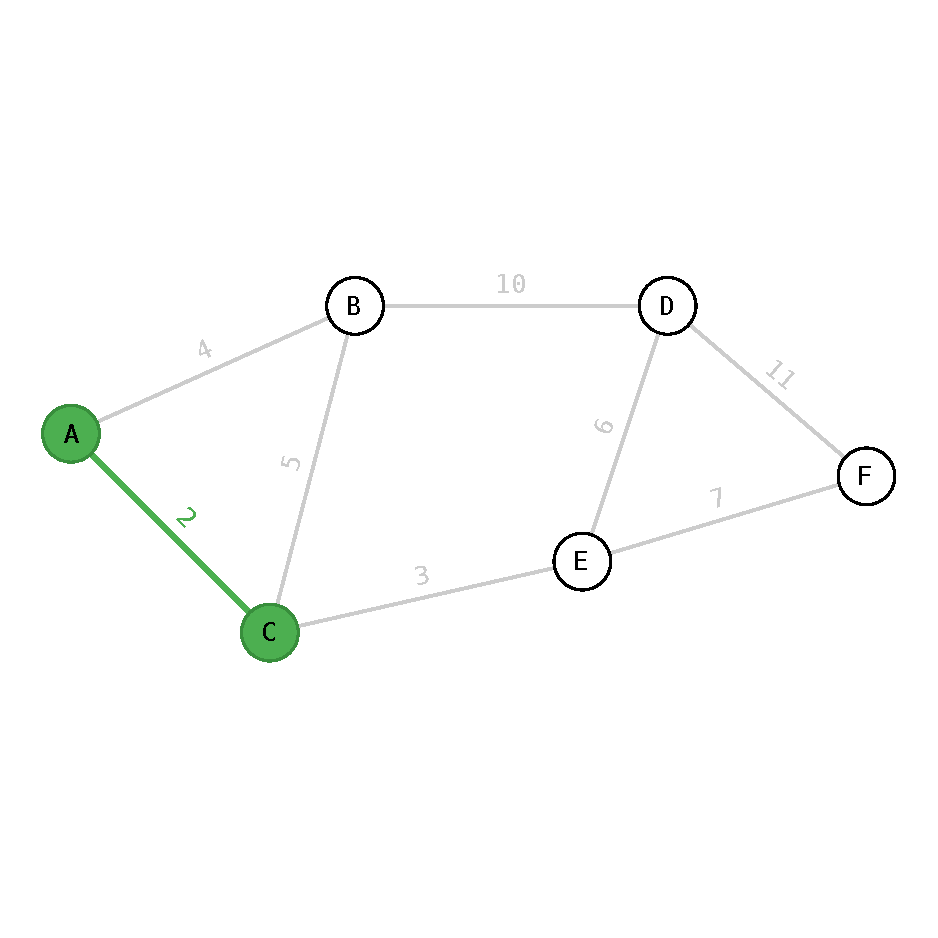
\includegraphics[width=0.30\textwidth]{python/lec07/prim_task/primt-1.pdf}\\[2pt]{\scriptsize $+AC(2)$}} &
\shortstack{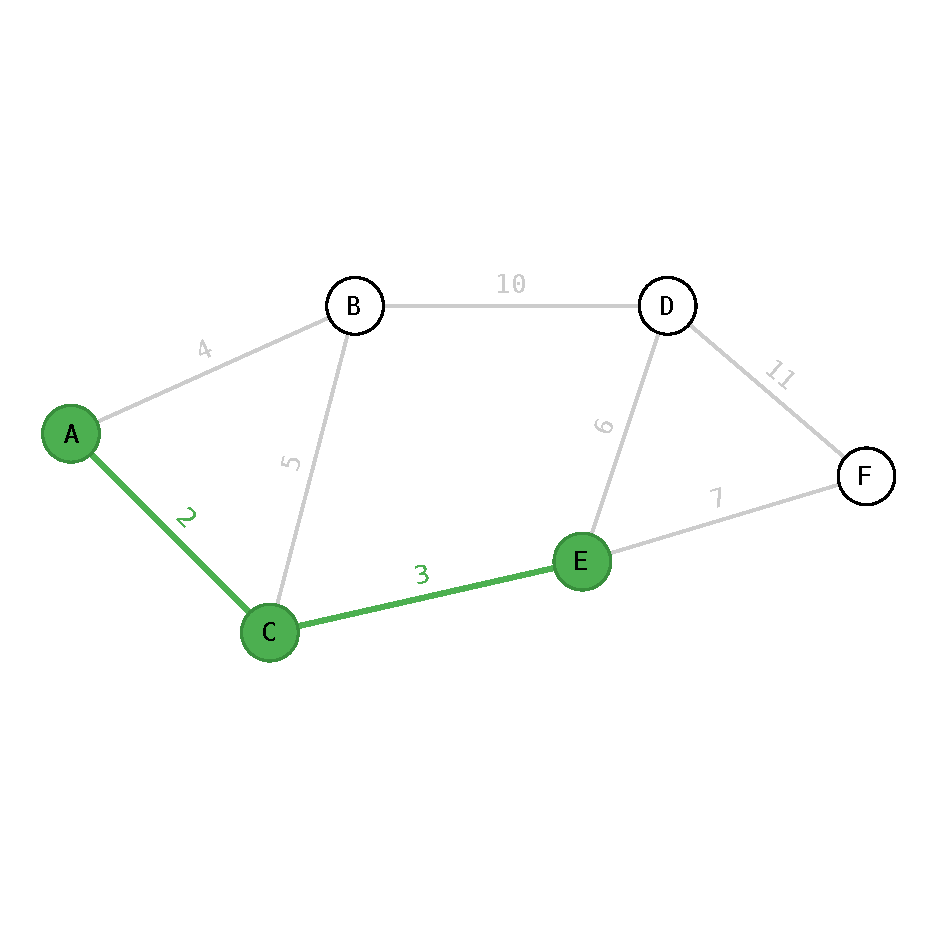
\includegraphics[width=0.30\textwidth]{python/lec07/prim_task/primt-2.pdf}\\[2pt]{\scriptsize $+CE(3)$}} &
\shortstack{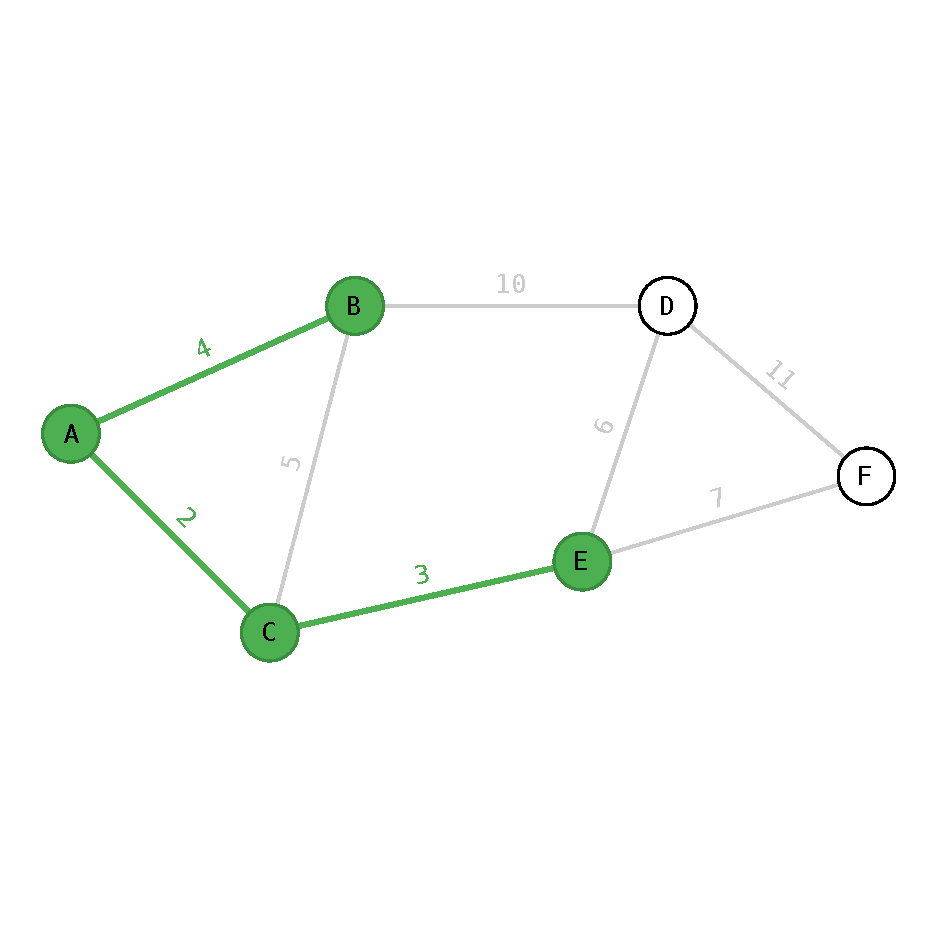
\includegraphics[width=0.30\textwidth]{python/lec07/prim_task/primt-3.pdf}\\[2pt]{\scriptsize $+AB(4)$}} \\
\end{tabular}\end{center}
\begin{center}\begin{tabular}{ccc}
\shortstack{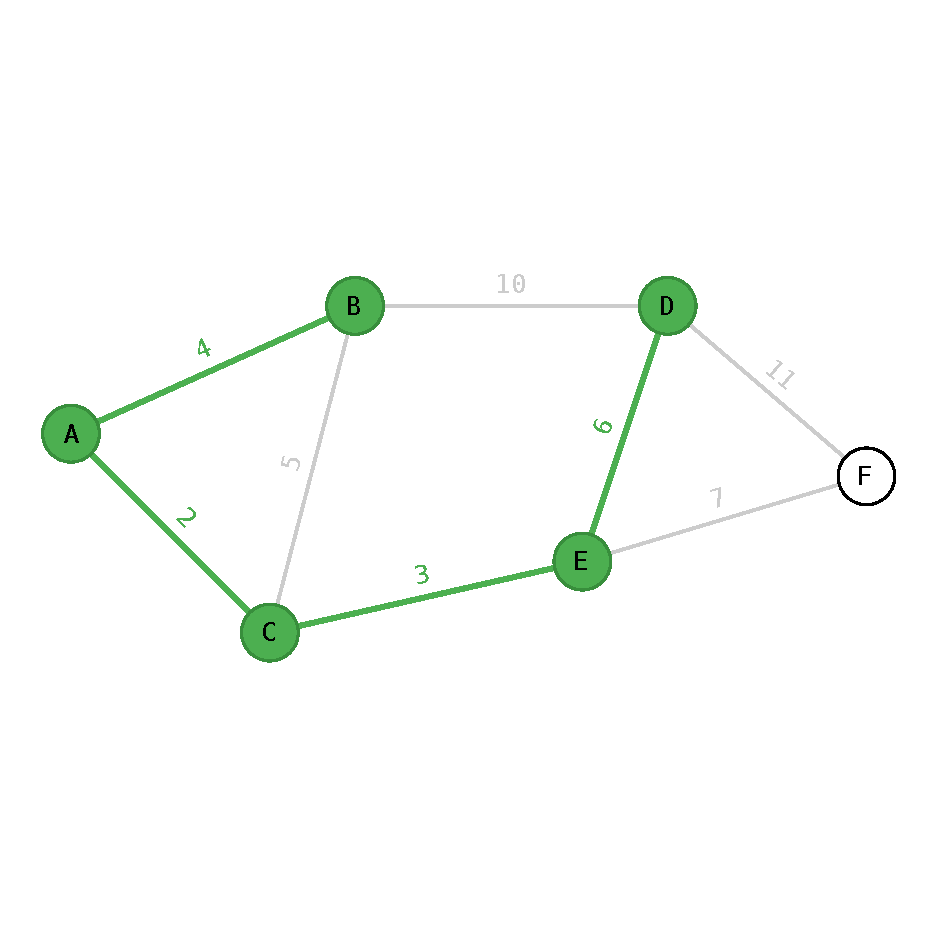
\includegraphics[width=0.30\textwidth]{python/lec07/prim_task/primt-4.pdf}\\[2pt]{\scriptsize $+ED(6)$}} &
\shortstack{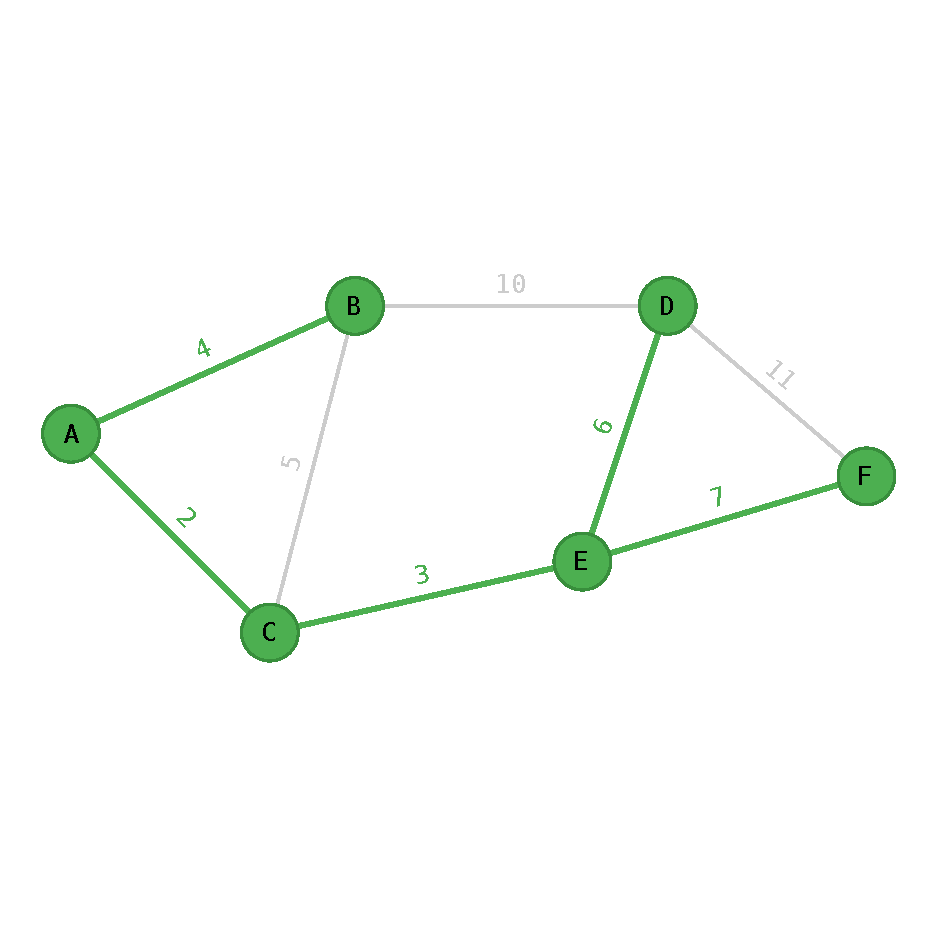
\includegraphics[width=0.30\textwidth]{python/lec07/prim_task/primt-5.pdf}\\[2pt]{\scriptsize $+EF(7)$}} &
\shortstack{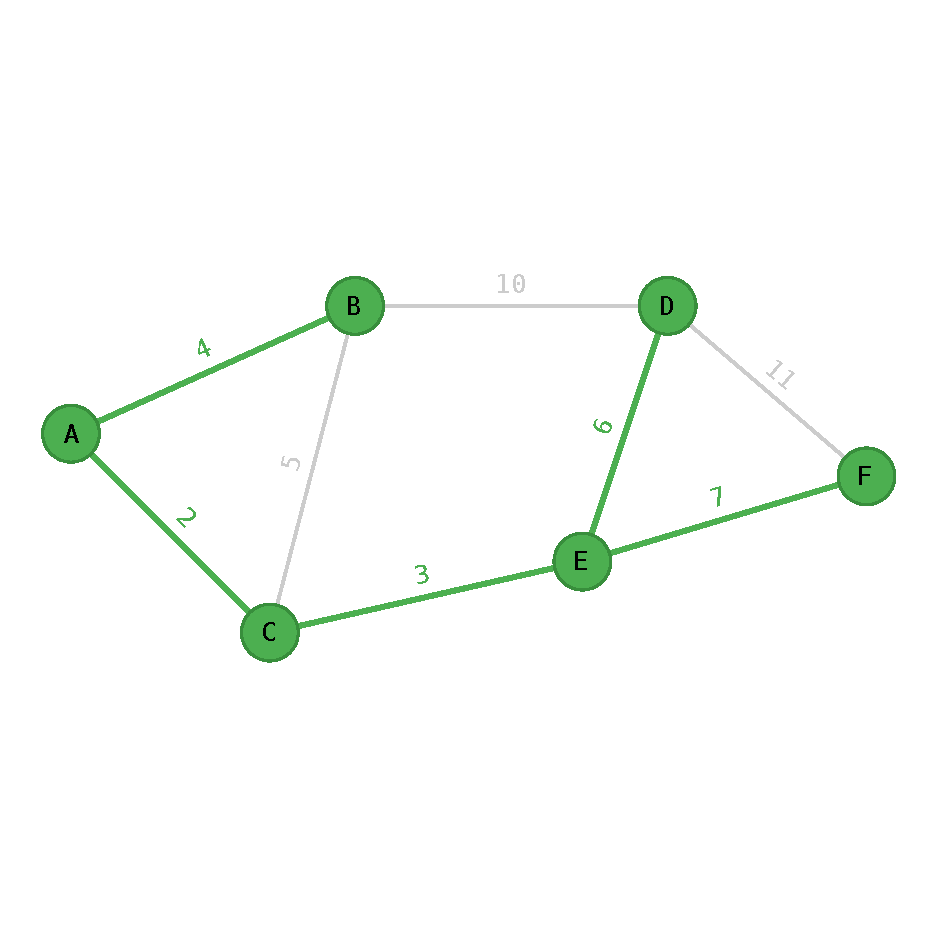
\includegraphics[width=0.30\textwidth]{python/lec07/prim_task/primt-6.pdf}\\[2pt]{\scriptsize Остов построен}} \\
\end{tabular}\end{center}

\textbf{Ответ.} Минимальное остовное дерево состоит из рёбер $AC,CE,AB,ED,EF$;
его суммарный вес равен $2+3+4+6+7=22$.
\end{task}
